\mode
<article>

\newpage

\mode
<all>

\mysection{Appendice}

\myframet{L'Europa nel 1600}{Europa 1600}{frame:europa1600}{
  \begin{center}
    \includegraphics[scale=0.25]{atlas/europe_map_1600.jpg}
  \end{center}
}

\myframet{Le company inglesi}{Companies}{frame:companies}{
  \begin{center}
    \includegraphics[scale=1.5]{atlas/companies-ok.png}
  \end{center}
}

\myframet{Il commercio veneziano}{Commercio}{frame:commveneziano}{
  \begin{center}
    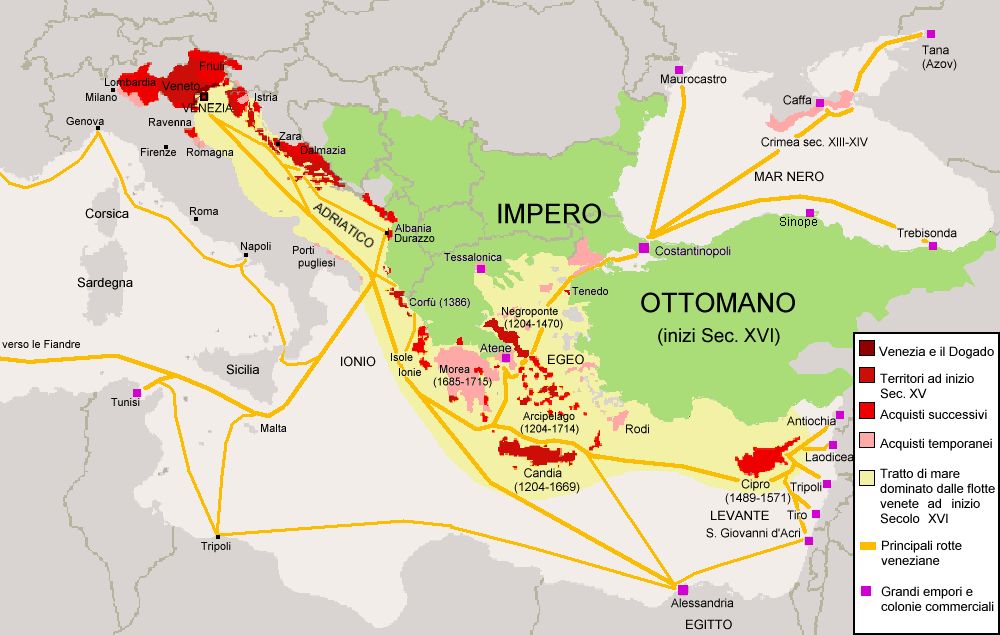
\includegraphics[scale=0.25]{atlas/Repubblica_di_Venezia.png}
  \end{center}
}

\myframet{L'economia mondo dei romani}{Romani}{frame:ecoromani}{
  \begin{center}
    \includegraphics{atlas/romani-ok.png}
  \end{center}
}

\myframe{La tessitura}{frame:tessitura}{
  \begin{center}
    \includegraphics[scale=0.45]{documenti/269tessitore.jpg}
  \end{center}
}

\myframet{Polizza del 1404}{Polizza 1404}{frame:polizza1404}{
  \begin{center}
    \parbox[c]{0.3\textwidth}{\includegraphics[scale=0.22]{documenti/docassic.png}}
    \hfill\parbox[c]{0.6\textwidth}{
      \begin{tabular}{p{0.59\textwidth}}
        ASGE,  {\it Notai  antichi} 523,  doc. 52\\  
        Chio,  11 gennaio 1404\\[2mm] 
        Ilario Cattaneo, Enrico Giustiniani Longo e Agostino Usodimare
        riconoscono di  avere ricevuto da Giovanni Podara  di Rodi del
        denaro, e  promettono di  consegnargli 500 ducati  d’oro entro
        sei mesi, se la nave  patronizzata da Costanzo Iarachi di Rodi
        approderà al porto di Costantinopoli.\\
      \end{tabular}
    }
  \end{center}
}

\myframet{Polizza prestampata del 1752}{Polizza 1752}{frame:polizza1752}{ 
  \begin{center}
    \includegraphics[scale=0.5]{documenti/Polizza-cadice-17520807.jpg}
  \end{center}
}

\myframet{Il declino della produzione a Bursa}{Declino Bursa}{frame:declinobursa}{
  \begin{center}
    \includegraphics[scale=0.25]{schemi/declinobursa.png}
  \end{center}
}

\myframet{Bilancio del governo centrale ottomano}{Bilancio}{frame:bilancio}{
  \begin{center}
    \includegraphics[scale=0.6]{schemi/pamuk133.png}
  \end{center}
}

\myframet{Rapporto tra akçe e altun}{Akçe/altun}{frame:rapportoakcealtun}{
  \begin{center}
    \includegraphics[scale=0.6]{schemi/pamuk136.png}
  \end{center}
}

\myframet{Rapporto con le monete europee}{Monete europee}{frame:rapportomoneuro}{
  \begin{center}
    \includegraphics[scale=0.6]{schemi/pamuk144.png}
  \end{center}
}

\myframe{Zecche ottomane}{frame:zecche}{
  \begin{center}
    \includegraphics[scale=0.5]{schemi/pamuk91.png}
  \end{center}
}

\myframe{Velocità delle lettere verso Venezia}{frame:lettere}{
  \begin{center}
    \includegraphics[scale=1.5]{atlas/lettere.png}

    \vspace{1cm}

    {\footnotesize Ogni isocrona rappresenta una settimana}

  \end{center}
}

